% Methodologie/Roberta.tex


\subsection{Utilisation de modèle pré-entraîné Roberta}

\subsubsection{Initialisation du Modèle RoBERTa pour l'Analyse de Sentiments}
\begin{figure}[h]
    \centering
    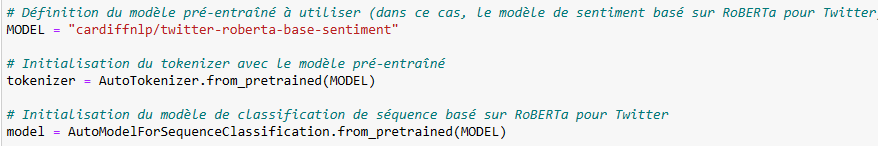
\includegraphics[scale=0.6]{assets/iniRoberta.PNG}
    \caption{initialisation de model RoBERTa}
    \label{fig:initroberta}
\end{figure}
Ces lignes de code définissent le modèle pré-entraîné à utiliser pour l'analyse de sentiments, en l'occurrence le modèle de sentiment basé sur RoBERTa pour Twitter. Le tokenizer associé au modèle est également initialisé, ainsi que le modèle de classification de séquence basé sur RoBERTa pour Twitter. Ces étapes préparent le modèle pour l'analyse ultérieure des sentiments dans le texte.


\subsubsection{Fonction d'Évaluation des Scores de RoBERTa pour l'Analyse de Sentiments}

\begin{figure}[h]
    \centering
    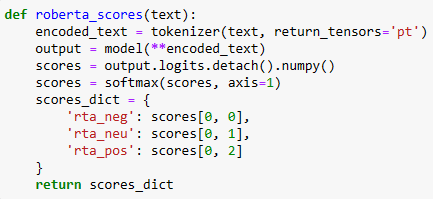
\includegraphics[scale=0.6]{assets/robertaFun.PNG}
    \caption{Fonction d'Évaluation des Scores de RoBERTa}
    \label{fig:evalfunroberta}
\end{figure}